\chapter{论文引用}

\section{引文相关}
此处的论文引用采用的是类似于IEEE的按出现位置的数字编号格式。建议将被引用的论文全名放入dblp网站(必应谷歌搜索dblp)搜索,之后进入该论文详细信息,如图~\ref{fig:dblpForBibtexCH7}所示。

\begin{figure}[htb]
  \centering
  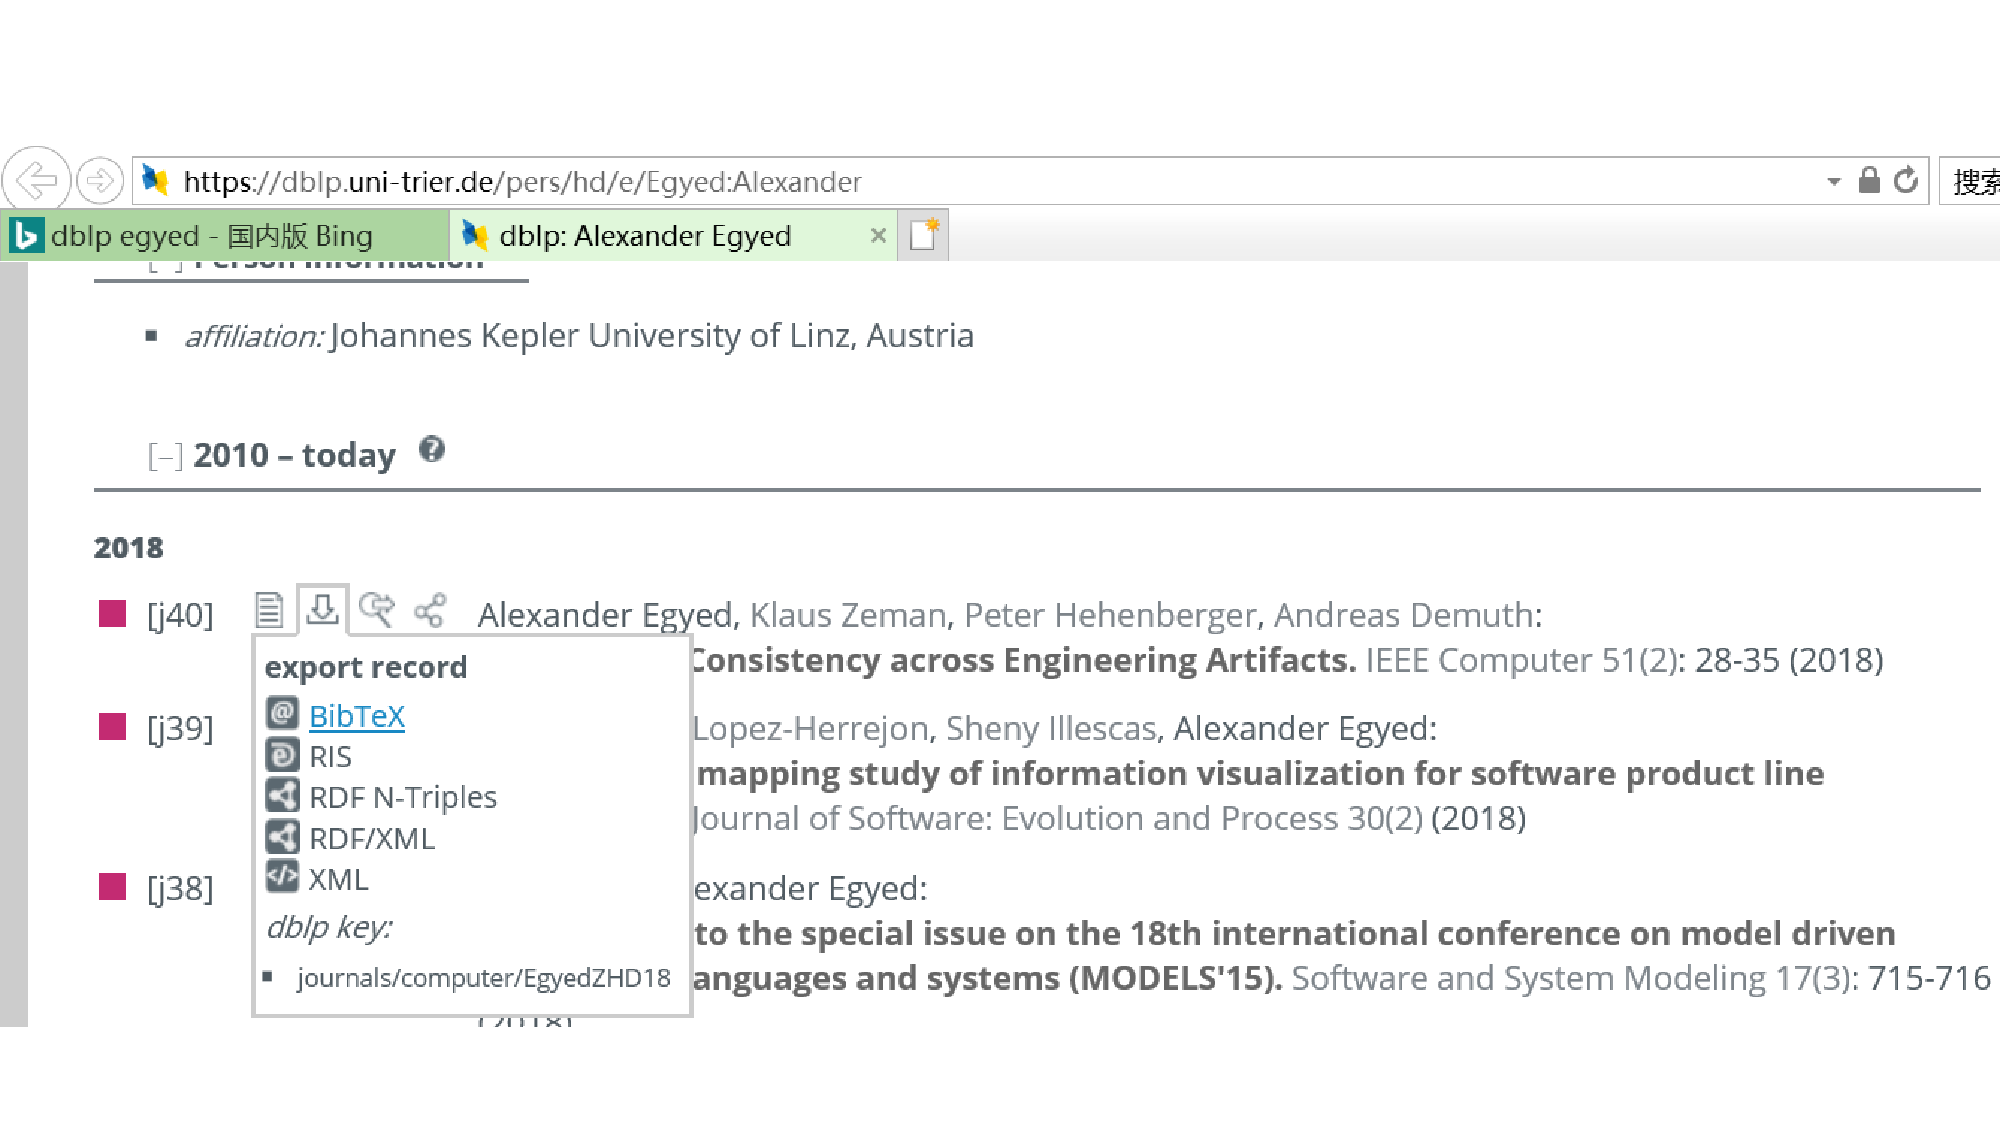
\includegraphics[width=5in]{figure/chapter7/dblpForBibtex.pdf}
  \caption{在dblp上下载Bibtex}
  \label{fig:dblpForBibtexCH7}
\end{figure}

点击图~\ref{fig:dblpForBibtexCH7}中所示的链接之后将得到Bibtex信息,如图~\ref{fig:bibtexDetailCH7}所示。
打开本地文件夹下的sample.bib文件,完整添加该信息。
并在需要引用的位置添加这一引用~\cite{DBLP:journals/computer/EgyedZHD18}。
格式为bibtex信息中的开头,\emph{例如图中的“DBLP:journals/computer/EgyedZHD18”。(此处是一个典型的因为长字符串导致的bad box,请参考上述章节的内容手动进行软换行)}。

\textbf{注意:在修改并保存sample.bib文件后,先编译tex文件,再编译参考文献,之后再编译两次,此时引用位置的方括号内将出现具体的编号而不是问号,且编号对应的引文已经出现在参考文献内。本模板点击引用编号后可以跳转到对应的参考文献处。}

在bib文件中出现,但并未在论文中被引用的论文不会出现在最后的参考文献中。如果dblp中并未包含你需要的论文,则可以尝试谷歌或百度学术的搜索结果,一般也包含bibtex信息,但可能不完整或不规范。

引用英文文献时,为了显示英文标注(例如“et al”“Vol”“ed”等),需要添加\texttt{language=\{en\}}属性。

引用网站链接可以考虑这一格式~\cite{GanttSystemWeb}(不推荐,网站链接使用脚注更规范些)。

引用书籍可以考虑这一格式~\cite{Pohl2010Requirements}。

中文文献请参考这一格式~\cite{cyg2006}。

以下英文引用用来测试引文排序是否按照插入顺序,以及多引文是否合并~\cite{DBLP:journals/computer/EgyedZHD18, DBLP:journals/ml/TingZCZWZ19}。

\begin{figure}[htb]
  \centering
  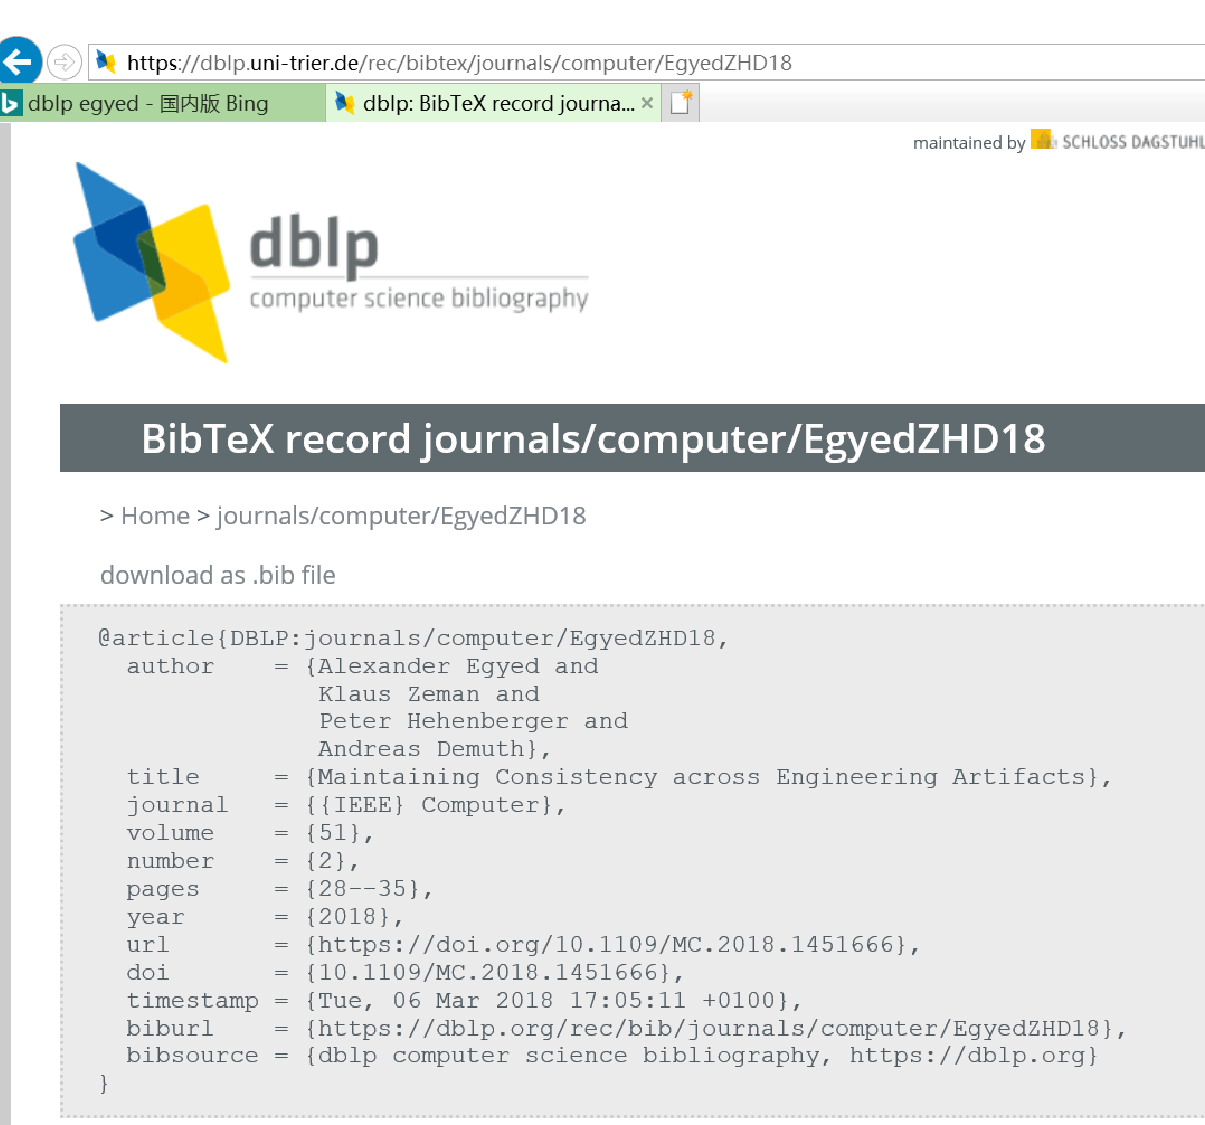
\includegraphics[width=5in]{figure/chapter7/bibtexDetail.pdf}
  \caption{Bibtex详细信息}
  \label{fig:bibtexDetailCH7}
\end{figure}
